\documentclass[12pt]{beamer}
\usepackage[utf8]{inputenc}
\usepackage{amsmath}
\usepackage{amsfonts}
\usepackage{amssymb}
\usepackage{graphicx}
\usepackage{alltt}
\graphicspath{{../sharedfiles/}}
%\usepackage[size=A4]{beamerposter}
\author{Anthony Odenthal, KE7OSN Amateur Extra}
\title{Technician and General Class Amateur Radio \& Satellite Stuff}
\AtBeginSection[]
{
\begin{frame}
\frametitle{Table of Contents}
\tableofcontents[currentsection]
\end{frame}
}
\AtBeginSubsection[]
{
  \begin{frame}
    \frametitle{Table of Contents}
    \tableofcontents[currentsection,currentsubsection]
  \end{frame}
}

\usetheme{PaloAlto}
\usecolortheme{beetle}

\begin{document}

\frame{\titlepage}

%\begin{frame}
%\frametitle{Table of Contents}
%\tableofcontents
%\end{frame}

\section{Introduction}

\begin{frame}
\frametitle{Welcome}
Welcome, over the next several sessions we will cover a substantial amount of information. please ask questions and slow me down.\\
The goals are:
\begin{itemize}
\item To introduce you to Amateur Radio \pause
\item Prepare you to take (and pass) the technician and general exams \pause
\item Introduce you to satellite communications.
\end{itemize}
\end{frame}

\begin{frame}
\frametitle{A little about myeself}
\begin{itemize}
%\item I'm a student at Oregon State University %Going to keep to just radio stuff
\item Passed Tech Sept 2007
\item Passed Gen Oct 2007
\item Joined Benton County ARES April 2012
\item Passed Extra April 2012
\item Became a VE in June 2012
\end{itemize}
\end{frame}

\begin{frame}
\frametitle{What is Amateur Radio?}
Amateur radio are people and activities that are regulated and encouraged, in the US and abroad, that allow licensed individuals to play around with radio waves, electronics, software, techniques, practices, and equipment to do all sorts of really cool stuff. Radio Amateurs are some of the least restricted users of radio spectrum, and with that freedom they have proven time and time again their worth.
The term Amateur refers to someone who does something as a pastime rather than a profession.
\end{frame}

\begin{frame}
\frametitle{Some useful tools}
Some things you may want to look into as useful for studying
\begin{itemize}
\item AA9PW practice exams \url{http://aa9pw.com}
\item ARRL license Manuals \url{http://www.arrl.org/shop/Licensing-Education-and-Training/}
\end{itemize}
\end{frame}

\begin{frame}
\frametitle{About the test}
\begin{itemize}
\item 35 questions \pause
\item Multiple Choice \pause
\item No time limit \pause
\item 396 questions in the tech pool, 457 in the general \pause
\item Need a 75\% to pass
\end{itemize}
\end{frame}

\begin{frame}
\frametitle{Shal we begin?}
Remember if I go too fast or you have questions, let me know.
\end{frame}

\section{General Rules}
%\subsection{T1A - Amateur Radio services; purpose of the amateur service, amateur-satellite service, operator/primary station license grant, where FCC rules are codified, basis and purpose of FCC rules, meanings of basic terms used in FCC rules}
\subsection{Who's In Charge}
\begin{frame}
\frametitle{Who's In charge}
International Telecommunications Union (ITU)
\begin{itemize}
\item Worldwide, treaty-based organization that allocates frequencies for specific uses.
\item Primary Users - first "rights" to a frequency
\item Secondary Users - permitted to use a frequency but must not interfere with a primary user
\item World divided into 3 regions, US is in Region 2
\item Creates "bands" - sections of spectrum allocated for amateur radio use.
\end{itemize}
\end{frame}

\begin{frame}
\frametitle{Who's In Charge}
Federal Comunications Commission (FCC)
\begin{itemize}
\item Promulgates  rules for non-federal radio users within ITU spec
\item Divides amateur bands into mode-specific sub-bands
\item Rules for telecommunications are in the Code of Federal Regulations, Chapter 47
\item Rules for amateur radio are in Part 97 of Chapter 47 (47 CFR 97)
\end{itemize}
\end{frame}

\begin{frame}
\frametitle{Who's In Charge}
Frequency Coordinator
\begin{itemize}
\item FCC recognized regional groups that coordinate the use of bands between large number of users \pause
\item Appointed by amateurs for amateurs \pause
\item Intended to help reduce and allow resolution of interference issues \pause
\item Voluntary rules unless there is interference, then the coordinated user "wins"\pause
\item Gentleman's agreement
\end{itemize}
\end{frame}

\begin{frame}
\frametitle{FCC allocations}
\begin{center}
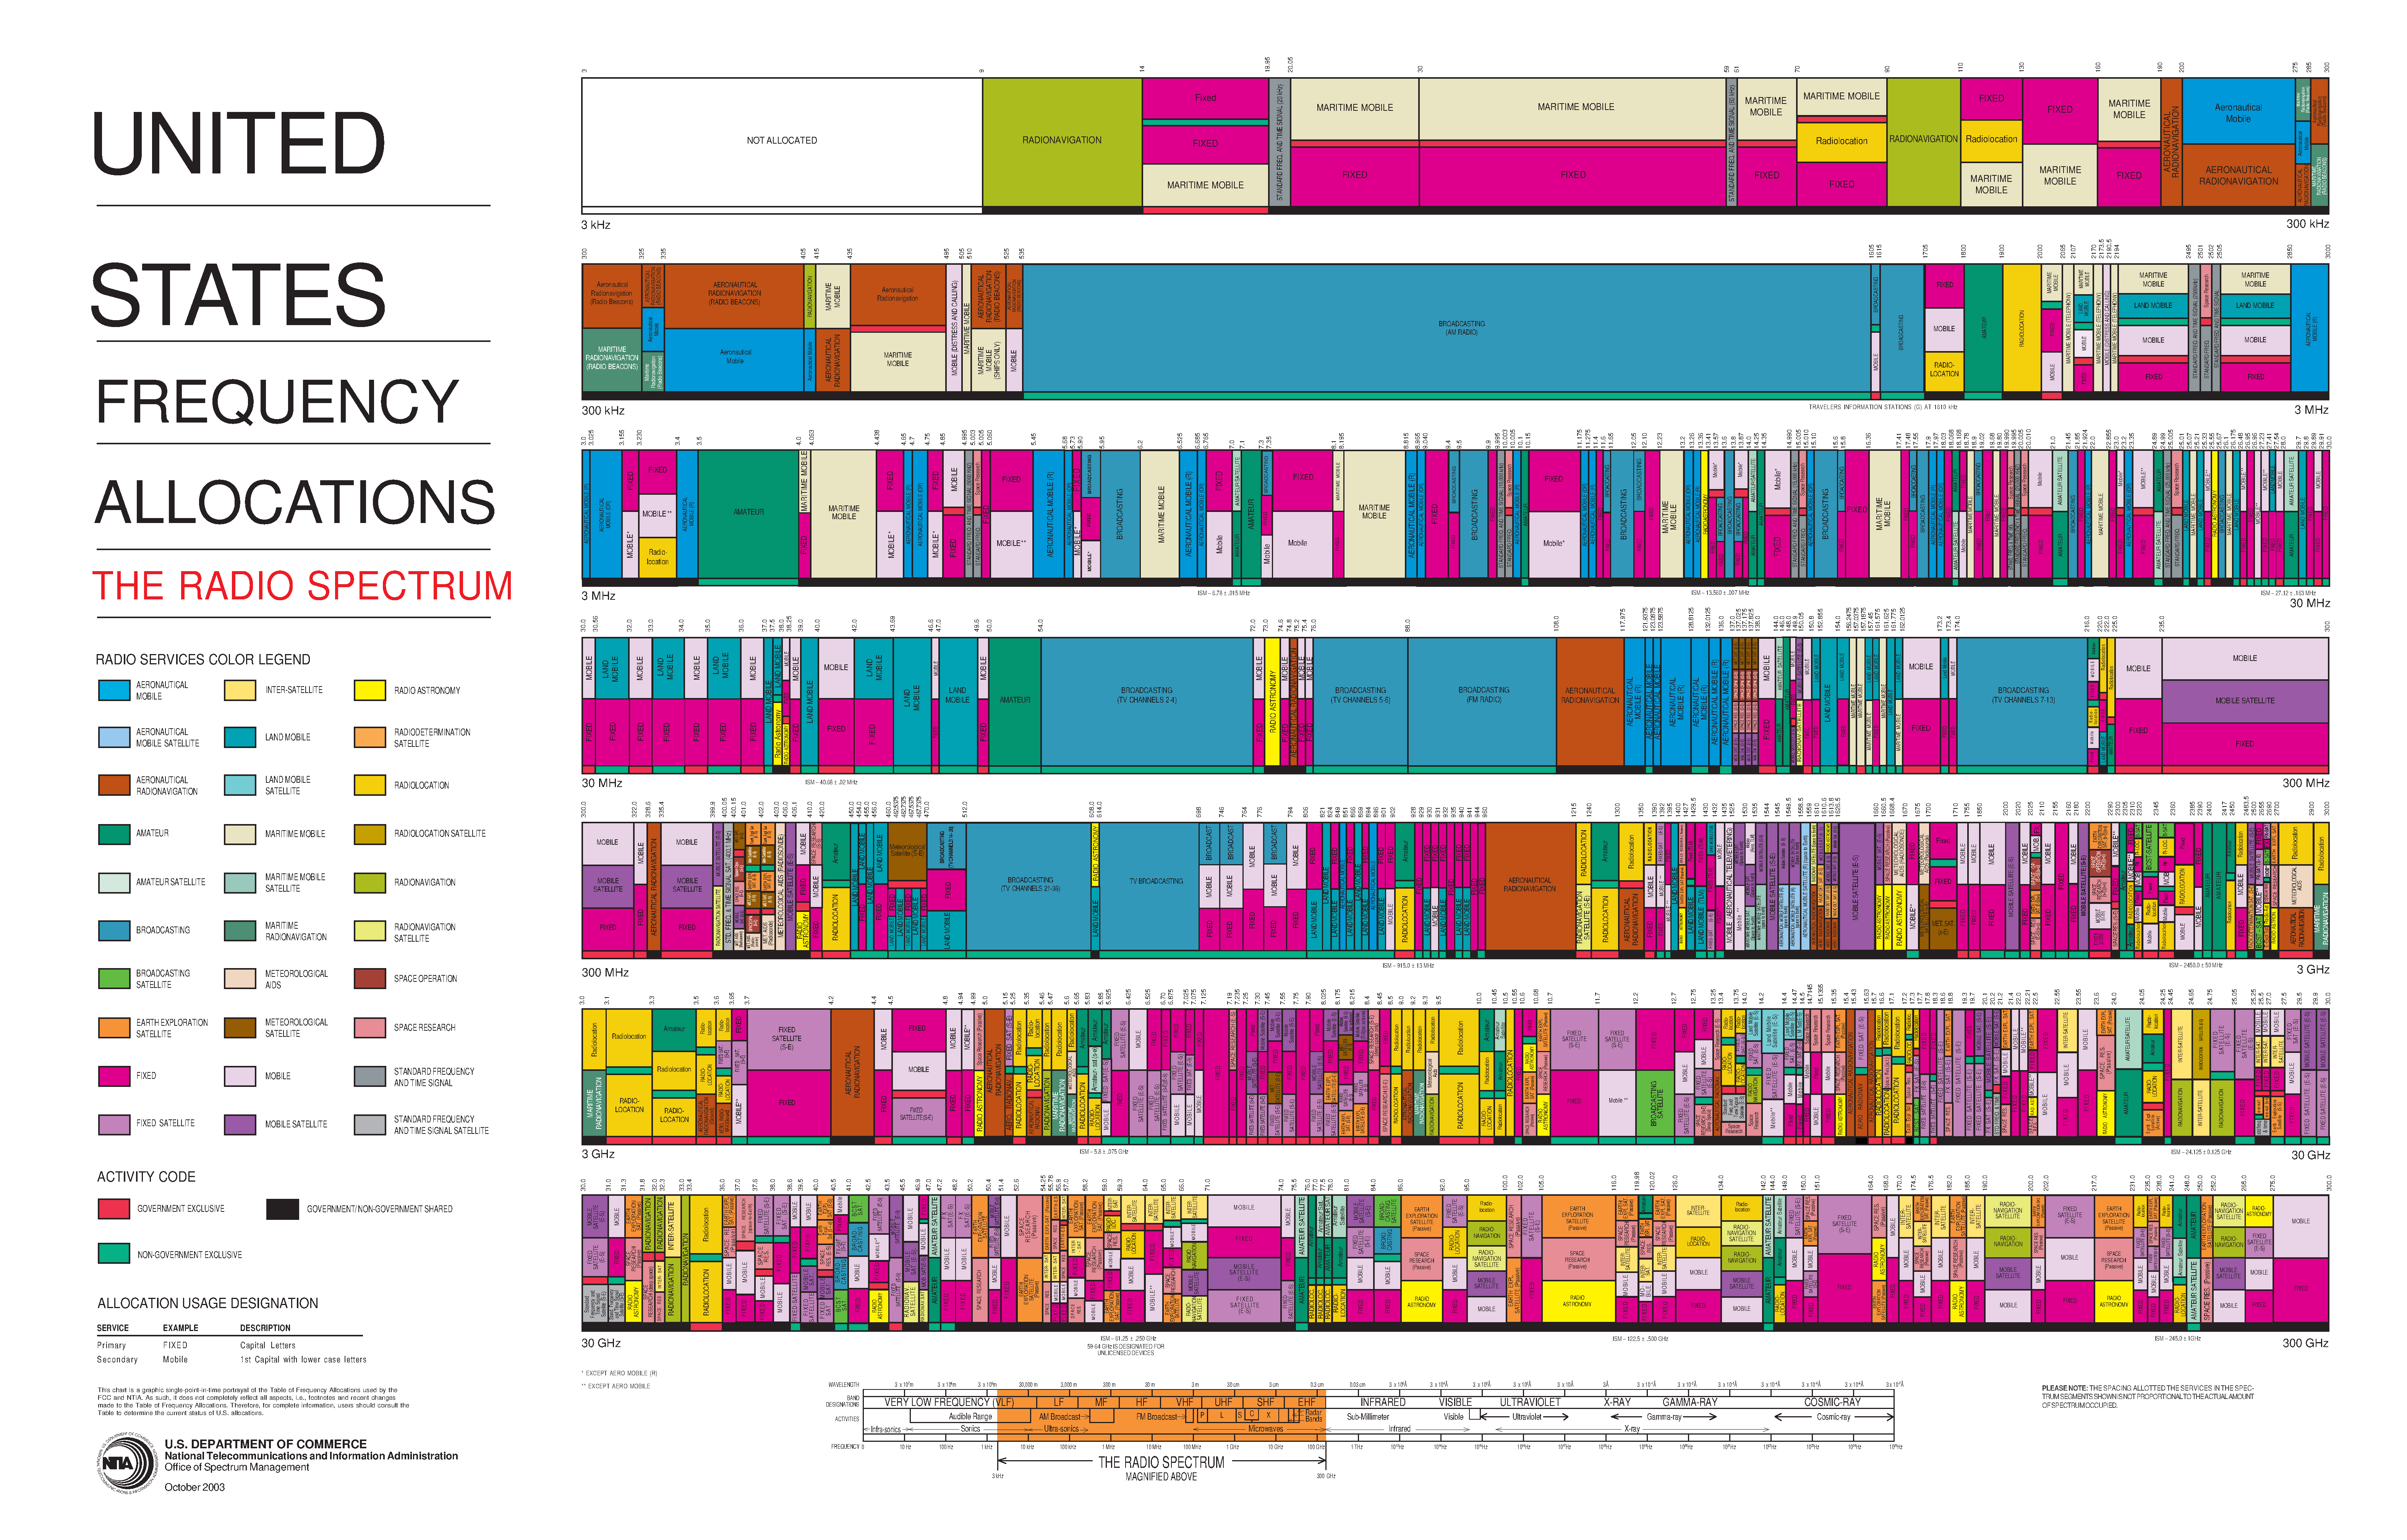
\includegraphics[width=\textwidth]{2003-allochrt.pdf}
\end{center}
\end{frame}

\subsection{Part 97}

\begin{frame}
\frametitle{47 CRF 97.1 Basic Purpose}
The rules and regulations in this part are designed to provide an amateur radio service having a fundamental purpose as expressed in the following principles:
\begin{enumerate}[A]
\scriptsize\item  Recognition and enhancement of the value of the amateur service to the public as a \emph{voluntary noncommercial communication service}, particularly with respect to providing emergency communications.\pause
\item Continuation and extension of the amateur's proven ability to contribute to the advancement of the radio art.\pause
\item Encouragement and improvement of the amateur service through rules which provide for advancing skills in both the communication and technical phases of the art.\pause
\item  Expansion of the existing reservoir within the amateur radio service of trained operators, technicians, and electronics experts. \pause
\item Continuation and extension of the amateur's unique ability to enhance international goodwill.
\end{enumerate}
\end{frame}

\begin{frame}
\frametitle{Keyphrase}
\begin{alltt}
\ldots\emph{a voluntary noncommercial\\communications service}\ldots
\end{alltt}
This phrase sums up almost every rule and tenant of amateur radio.
\end{frame}

\begin{frame}
\frametitle{A voluntary noncommercial communications service}
Noncommercial means no "pecuniary interest". It is illegal to profit from the use of amateur radio.\\
\hfil \\As with almost any rule there are exceptions"
\begin{itemize}
\item Teachers may use ham radio in the classroom as a teaching aid
\item "Code practice" transmissions
\item Disaster Drills
\end{itemize}
\end{frame}

\begin{frame}
\frametitle{More basic rules}
\begin{itemize}
\item No Music - expect transmission or re-transmission of a signal from a space station
\item No Broadcasting
\item No commercial traffic
\item No profanity
\item No codes or ciphers intended to hid content
\item No international third party traffic unless treaty-approved
\end{itemize}
\end{frame}

\subsection{licenses}

\begin{frame}
\frametitle{Licenses}
A license is valid for ten years, with a two year grace period. Upgrades don't count as renewals. Basic renewals are free!\\
There are five classes.
\begin{itemize}
\item *Novice
\item Technician
\item General
\item *Advanced
\item Extra
\end{itemize}
\end{frame}

\begin{frame}
\frametitle{Licenses}
There are four kinds of licenses, Individual hams hold both a "Station" and "Operator"
\begin{itemize}
\item Station
\item Operator
\item Club - W7OSU, K7CVO, W1AW
\item Special Event - A7W
\end{itemize}
Clubs can get a "club callsign", and events can get an event callsign.
\end{frame}

\subsection{Callsigns}

\begin{frame}
\frametitle{Callsigns}
\begin{itemize}
\item US callsigns start with A,K,N, or W
\item The format is one or two letters, a number, and one to three letters.
\item New callsigns are assigned in sequential order - number indicates the region in the US
\item Shorter callsigns are reserved for higher license classes
\item 1X1 for special events only
\end{itemize}
\end{frame}

\begin{frame}
\frametitle{Callsigns}
\begin{itemize}
\item KE7OSN \pause
\item N8GFO \pause -Yep \pause
\item K7HZ \pause -That's an Extra \pause
\item VE6GLW \pause -That's Canadian, eh\pause
\item KLOO \pause -That's a commercial station \pause
\item WSJ509 \pause -Land Mobile, Benton County Sheriff \pause
\item Mission Base \pause -What is known as a "tactical callsign"
\end{itemize}
\end{frame}

\begin{frame}
\frametitle{What IS an amateur station?}
T1A10 (A) [97.3(a)(5)] What is the FCC Part 97 definition of an amateur station?\\ \pause \hfil \\
A. A station in an Amateur Radio Service consisting of the apparatus necessary for carrying on radio
communications
\end{frame}

\begin{frame}
\frametitle{Operator}
Who "operates" an amateur station? \pause \\
The control operator, who is designated by the station licensee, and determines the privileges of operation.\\
e.g.\ if you are at a radio that can operate outside your privileges, you still can only use what you are licensed to.
\end{frame}

\begin{frame}
\frametitle{Your Callsign}
A station must transmit it's callsign at least every ten minutes and at the end of every communication.\\
Special situations have special rules\\
\begin{itemize}
\item Control operator working outside of a station licensee privileges.
\item Special event station control operator
\item Control operator using new privileges prior to FCC database update
\end{itemize}
\end{frame}

\begin{frame}
\frametitle{The Uniform Licensing System}
The ULS is an online database of FCC license information. A new licensee may use their privileges as soon as their information appears in the ULS. When you upgrade you may use your new privileges as soon as you pass the test.
\end{frame}

\begin{frame}
\frametitle{Typical uses of a callsign}
\begin{itemize}
\item W7OSU This is KE7OSN \pause
\item Net Control This is KE7OSN \pause
\item This is W7OSU (Go Ahead) \pause
\item CQ CQ CQ this is KE7OSN \pause
\item KE7OSN monitoring \pause
\item This is KF7FGE stroke (/) KE7OSN \pause
\item Hey Bob, you around?
\end{itemize}
\end{frame}

\begin{frame}
\frametitle{Hey bob, you around}
Hey bob you around?\\
Legal? \\ \pause
Yes, as long as you keep to the every ten minutes and the end of every communication. \\ \pause
What if Bob isn't there? \\ \pause
KE7OSN clear
\end{frame}

\begin{frame}
\frametitle{Types of stations}
\begin{itemize}
\item Club – at least four  people, one of which accepts responsibility and is the “trustee”.
\item Space – at least 50km above the surface.
\item Beacon --  transmits a low-level signal for propagation studies
\item Repeater – retransmits  a signal heard on one frequency on another frequency.
\item Auxillary – a secondary receiver that feeds a repeater station.  
\end{itemize}
\end{frame}

\subsection{frequencies}

\begin{frame}
\frametitle{Band Plan}
\begin{center}
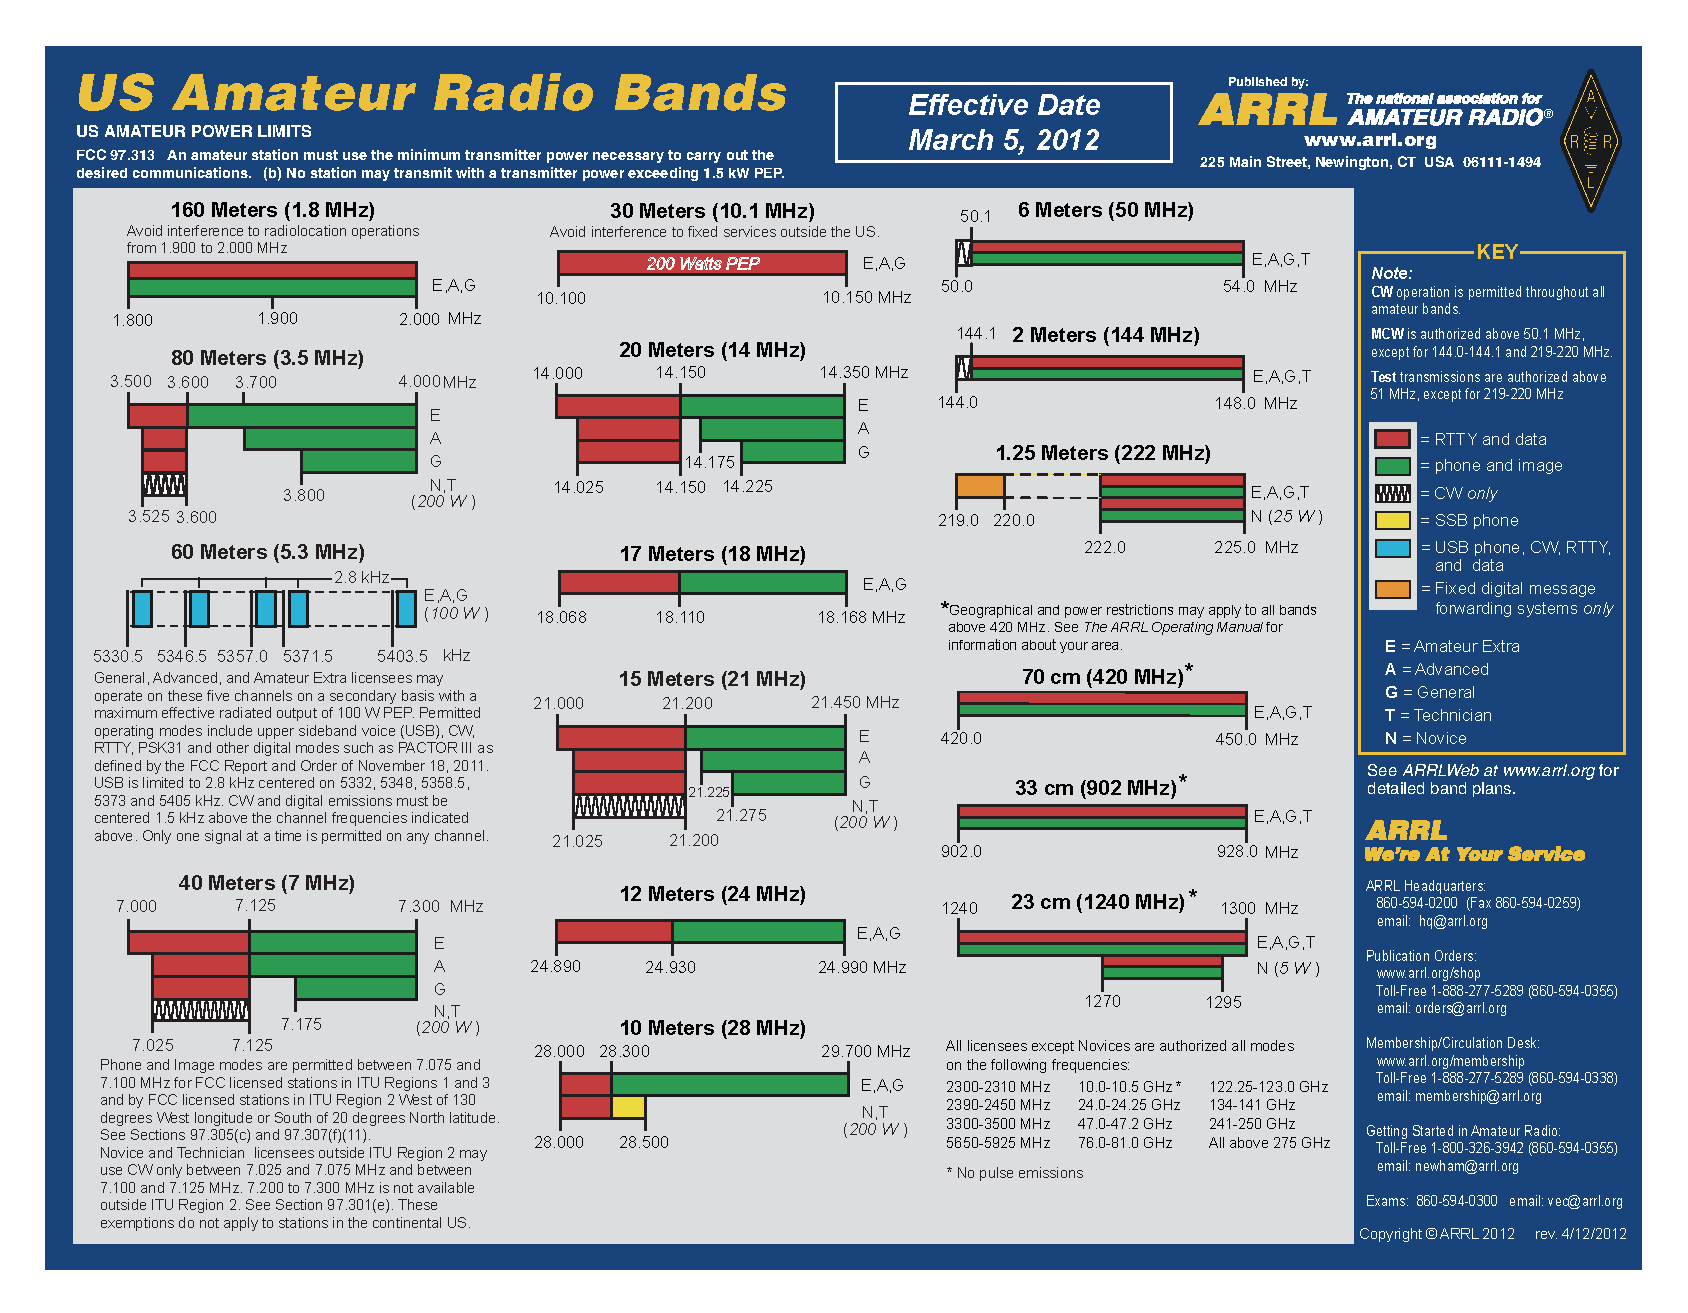
\includegraphics[width=\textwidth]{hambandscolor.pdf}
\end{center}
\end{frame}

\begin{frame}
\frametitle{ITU Band Names}
\begin{itemize}
\item MF - Medium Frequency 300KHz to 3MHz
\item HF - High Frequency 3MHz to 30 MHz
\item VHF - Very High Frequency 30MHz to 300MHz
\item UHF - Ultra High Frequency 300MHz to 3GHz
\item SHF - Super High Frequency 3GHz to 30GHz
\item EFE - Extremely High Frequency - 30GHz to 300GHz
\item THF - Tremendously High Frequency - 300GHZ to 3THz
\end{itemize}
\end{frame}

\begin{frame}
\frametitle{HF 3-30MHz}
	\begin{itemize}
	\item 80 Meters
		\begin{itemize}
		\item 3.525-3.600MHz: CW Only
		\end{itemize}
	\item 40 Meters
		\begin{itemize}
		\item 7.025-.125MHz: CW Only
		\end{itemize}
	\item 15 Meters
		\begin{itemize}
		\item 21.025-21.200MHz: CW Only
		\end{itemize}
	\item 10 Meters 
		\begin{itemize}
		\item  28.000-28.300MHz: CW, RTTY/Data 200 watts PEP max 
		\item 28.300-28.500MHz: CW, Phone 200 watts PEP max
		\end{itemize}
	\end{itemize}
\end{frame}

\begin{frame}
\frametitle{VHF 30-300MHz}
	\begin{itemize}
	\item 6 Meters
		\begin{itemize}
		\item 50.0-50.1MHz CW Only
		\item 50.1-54.0MHz All modes
		\end{itemize}
	\item 2 Meters
		\begin{itemize}
		\item  144.0-144.1MHz CW Only
		\item 144.1-148.0MHz All modes
		\end{itemize}
	\item 1.25 Meters
		\begin{itemize}
		\item 222.00-225.00MHz All modes
		\end{itemize}
	\end{itemize}
\end{frame}

\begin{frame}
\frametitle{UHF 300-3000MHz (3GHz)}
\begin{itemize}
\item 70 Centimeters
\begin{itemize}
\item 420.0-450.0MHz All Modes
\end{itemize}
\item 33 Centimeters
\begin{itemize}
\item 902.0-928.0MHz All Modes
\end{itemize}
\item 23 Centimeters
\begin{itemize}
\item 1240-1300MHz All Modes
\end{itemize}
\item 2.4GHz
\begin{itemize}
\item 2.3-2.31GHz
\item 2.39-2.45GHz *
\end{itemize}
\end{itemize}
\end{frame}

\begin{frame}
\frametitle{2.4GHz}
We share the 2390-2450MHz band with: 802.11 networks, cordless phones, video cameras, zigbee, etc.\ \\
We are PRIMARY users. We have first "rights". Secondary users must not cause us interference and must accept interference from our operations.
\end{frame}

\begin{frame}
\frametitle{SHF 3GHz-30GHz and up}
\begin{itemize}
\item 3.3-3.5GHz
\item  5.65-5.925GHz
\item  10.0-10.5GHz
\item  24.0-24.25GHz
\item  47.0-47.2GHz
\item  76.0-81.9GHz
\item  119.98-120.02GHz
\item  142-149GHz
\item  241-250GHz
\item  Everything above 300GHz
\end{itemize}
\end{frame}

\subsection{Questions}

\begin{frame}
\frametitle{T1A}
\begin{description}
\scriptsize\item[T1A01 (D) [97.3(a)(4)] For whom is the Amateur Radio Service intended?]\hfil \\D. Persons who are interested in radio technique solely with a personal aim and without pecuniary interest \pause

\item[T1A02 (C) [97.1] What agency regulates and enforces the rules for the Amateur Radio Service in the United States?] \hfil \\ C. The FCC \pause

\item[T1A03 (D) Which part of the FCC rules contains the rules and regulations governing the Amateur Radio Service?]\hfil \\ D. Part 97 \pause

\item[T1A04 (C) [97.3(a)(23)] Which of the following meets the FCC definition of harmful interference?]\pause \hfil \\ C. That which seriously degrades, obstructs, or repeatedly interrupts a radio communication service operating in accordance with the Radio Regulations \pause

\item[T1A05 (D) [97.3(a)(40)] What is the FCC Part 97 definition of a space station?] \hfil \\  D. An amateur station located more than 50 km above the Earth’s surface \pause

\item[T1A06 (C) [97.3(a)(43)] What is the FCC Part 97 definition of telecommand?]\hfil \\  C. A one-way transmission to initiate, modify or terminate functions of a device at a distance \pause
\end{description}
\end{frame}

\begin{frame}
\frametitle{T1A}
\begin{description}
\scriptsize
\item[T1A07 (C) [97.3(a)(45)] What is the FCC Part 97 definition of telemetry?]\hfil \\ C. A one-way transmission of measurements at a distance from the measuring instrument  \pause

\item[T1A08 (B) [97.3(a)(22)] Which of the following entities recommends transmit/receive channels and other parameters for auxiliary and repeater stations?]\hfil \\  B. Frequency Coordinator \pause

\item[T1A09 (C) [97.3(a)(22)] Who selects a Frequency Coordinator?]\hfil \\ C. Amateur operators in a local or regional area whose stations are eligible to be auxiliary or repeater stations  \pause

\item[T1A10 (A) [97.3(a)(5)] What is the FCC Part 97 definition of an amateur station?]\hfil A. A station in an Amateur Radio Service consisting of the apparatus necessary for carrying on radio communications \pause

\item[T1A11 (C) [97.3(a)(7)] Which of the following stations transmits signals over the air from a remotereceive site to a repeater for retransmission?] \hfil \\C. Auxiliary station
\end{description}
\end{frame}

\begin{frame}
\frametitle{Title}
hello world
\end{frame}

\begin{frame}
\frametitle{Title}
hello world
\end{frame}
\section{Emergency Operations}
\begin{frame}
\frametitle{Title}
hello world
\end{frame}

\begin{frame}
\frametitle{Title}
hello world
\end{frame}

\begin{frame}
\frametitle{Title}
hello world
\end{frame}

\begin{frame}
\frametitle{Title}
hello world
\end{frame}

\begin{frame}
\frametitle{Title}
hello world
\end{frame}

\begin{frame}
\frametitle{Title}
hello world
\end{frame}

\begin{frame}
\frametitle{Title}
hello world
\end{frame}

\begin{frame}
\frametitle{Title}
hello world
\end{frame}

\begin{frame}
\frametitle{Title}
hello world
\end{frame}

\begin{frame}
\frametitle{Title}
hello world
\end{frame}

\begin{frame}
\frametitle{Title}
hello world
\end{frame}

\begin{frame}
\frametitle{Title}
hello world
\end{frame}

\begin{frame}
\frametitle{Title}
hello world
\end{frame}

\begin{frame}
\frametitle{Title}
hello world
\end{frame}

\begin{frame}
\frametitle{Title}
hello world
\end{frame}

\begin{frame}
\frametitle{Title}
hello world
\end{frame}

\begin{frame}
\frametitle{Title}
hello world
\end{frame}

\begin{frame}
\frametitle{Title}
hello world
\end{frame}

\begin{frame}
\frametitle{Title}
hello world
\end{frame}

\begin{frame}
\frametitle{Title}
hello world
\end{frame}

\begin{frame}
\frametitle{Title}
hello world
\end{frame}

\begin{frame}
\frametitle{Title}
hello world
\end{frame}

\begin{frame}
\frametitle{Title}
hello world
\end{frame}

\begin{frame}
\frametitle{Title}
hello world
\end{frame}

\begin{frame}
\frametitle{Title}
hello world
\end{frame}

\begin{frame}
\frametitle{Title}
hello world
\end{frame}

\begin{frame}
\frametitle{Title}
hello world
\end{frame}

%
%\begin{frame}
%\frametitle{Title}
%hello world
%\end{frame}
%
\end{document}